\chapter{THEORIE DE CO-OCCURRENCE DES ESPECES DANS LES RÉSEAUX D'INTERACTION}
\label{chap2}

\section{Résumé en français du deuxième article}


\subsection{Contexte scientifique}

Au chapitre précédent, j'ai mis en évidence les impacts potentiels des interactions sur la présence locale des espèces dans le cadre de la TIB. Afin de faire un pas en avant vers le traitement des données typiques en biogéographie, les données de présence et d'absence des espèces, je me suis confronté aux problèmes de co-occurrence des espèces en interactions.

La co-occurence observée dans les données est simplement le nombre total de sites où les espèces sont présentes ensemble rapporté au nombre total de sites étudiés. Pour pouvoir aller plus loin, avec mes collaborateurs, nous avons défini une mesure de co-occurence sous l'hypothèse d'indépendance. Cela signifie que nous prenons l'occurrence respective des deux espèces et que nous les multiplions pour obtenir la mesure de co-occurrence sous cette hypothèse. Grâce à la comparaison entre ces deux valeurs nous avons été capables d'illustrer, dans l'article présenté ci-dessous, cinq grands principes relatifs à la co-occurence des espèces en interaction~:

1. \textbf{Les interactions directes entre deux espèces affectent la co-occurence}. C'est une transposition directe des résultats du chapitre précédent sur la mesure de co-occurrence~: s'il existe un lien entre deux espèces, leur probabilité d'être présentes simultanément dans une localité diffère de la probabilité attendue si elle se rencontraient aléatoirement.

2. \textbf{Les interactions indirectes modifient la probabilité de co-occurence}. Malgré l'absence d'interaction directe entre deux espèces, ces dernières peuvent néanmoins être liées par une ou plusieurs autres espèces, l'interaction est alors qualifiée d'indirecte. Si les conséquences des interactions directes se propagent à travers le réseau via ces relations indirectes, il est alors possible que la répartition d'une espèce soit affectée par une autre espèce avec laquelle aucune interaction directe n'est constatée.

3. \textbf{L'effet des interactions sur la co-occurrence n'est pas symétrique}. Il n'existe a priori aucune raison pour que ces effets soient symétriques. Néanmoins, en utilisant la mesure de co-occurrence telle que décrite ci-dessus, nous la considérons comme telle. Nous montrons alors comment les probabilités conditionnelles peuvent prendre en compte l'asymétrie des effets des interactions.

4. \textbf{La force d'association entre deux espèces diminue avec la longueur du plus court chemin entre deux espèces}. Plus les espèces sont éloignées dans le réseau, moins les conséquences des interactions indirectes seront perceptibles, nous montrons alors que les effets des interactions directes diminuent lors de leur propagation dans le réseau.

5. \textbf{La force d'une association avec une autre espèce diminue avec le nombre d'interaction qu'elle entretient.} Si une espèce a de nombreux liens dans le réseau (par exemple, un prédateur généraliste), alors celle-ci sera moins dépendante d'une espèce en particulier et de fait la relation qu'elle entretien avec les espèces se rapprochera de la co-occurrence sous hypothèse d'indépendance.

\subsection{Publication associée}

Pour ce second article, le contexte est particulier~: Dominique Gravel a été invité à un numéro spécial de la revue scientifique \textit{Theoretical Ecology} sur les réseaux écologiques. Dominique Gravel m'a alors proposé de travailler sur le prolongement de la réflexion menée au chapitre \ref{chap1} et de l'appliquer sur les données de co-occurrence. J'ai alors conceptualisé un modèle probabiliste pour tenter de comprendre comment les interactions peuvent affecter la co-occurrence. Je me suis occupé de toute la partie modèle et des figures. Avec Dominique Gravel, nous avons rédigé l'essentiel du manuscrit avec des apports significatifs de Nicolas Mouquet et de  Miguel B. Ara\'ujo qui sont alors devenus co-auteurs.
L'aricle a été publié en ligne en octobre 2015 et est sortie dans le volume 9
(volume de l'année 2016), le DOI associé est :
\textbf{10.1007/s12080-015-0281-9} \citep{Cazelles2016}.

\subsection{Traduction du résumé de l'article publié}

L'étude de la co-occurrence des espèces a été essentielle en écologie des communautés depuis la fondation de la discipline. Cependant, les données de co-occurence sont une source d'information négligée par les modèles de distribution d'espèces et les biogéographes se demandent encore quels sont les effets des interactions aux différentes échelles biogéographiques. Nous soutenons l'idée qu'une théorie de la co-occurrence des espèces au sein d'un réseau écologique est nécessaire pour mieux interpréter les données de co-occurrence, pour formuler des hypothèses sur les mécanismes d'assemblage des communautés et pour étendre l'analyse des distributions d'espèces qui se concentre actuellement sur la relation entre les données d'occurrences et les facteurs abiotiques. L'objectif principal de cet article est de fournir les premières briques d'une théorie générale de la co-occurrence des espèces. Nous formalisons le problème avec différentes probabilités étudiées dans un contexte d'analyse de co-occurrence. Nous analysons les modules de trois espèces en interactions et nous conduisons des simulations pour documenter cinq principes influençant les associations au sein d'un réseau écologique~: i) les interactions directes affectent la co-occurrence ii); les interactions indirectes affectent la co-occurrence; iii) la co-occurence est rarement symétrique; iv) la force d'une association diminue avec la longueur du chemin le plus court entre deux espèces; v) la force d'une association diminue avec le nombre d'interaction qu'une espèce entretient. Nos analyses révèlent la difficulté d'interprétation des interactions entre espèces avec des données de co-occurrence. Nous discutons la possibilité d'inférence de la structure des réseaux d'interaction depuis ces données. Nous argumentons également que les modèles de distribution peuvent bénéficier de l'incorporation des probabilités conditionnelles en vue d'intégrer la contribution des interactions biotiques dans la distribution d'une seule espèce.


\emph{Les sections qui suivent sont celles de l'article publié.}





\section{Titre}

A Theory for species co-occurrence in interaction networks

\section{Auteurs}

Kévin Cazelles, Miguel Ara\'ujo, Nicolas Mouquet et Dominique Gravel

\section{Résumé en anglais}

The study of species co-occurrences has been central in community ecology since the foundation of the discipline. Co-occurrence data are, nevertheless, a neglected source of information to model species distributions and biogeographers are still debating about the impact of biotic interactions on species distributions across geographical scales. We argue that a theory of species co-occurrence in ecological networks is needed to better inform interpretation of co-occurrence data, to formulate hypotheses for different community assembly mechanisms, and to extend the analysis of species distributions currently focused on the relationship between occurrences and abiotic factors. The main objective of this paper is to provide the first building blocks of a general theory for species co-occurrences. We formalize the problem with definitions of the different probabilities that are studied in the context of co-occurrence analyses. We analyse three species interactions modules and conduct multi-species simulations in order to document five principles influencing the associations between  species within an ecological network: i) direct interactions impact pairwise co-occurrence; ii) indirect interactions impact pairwise co-occurrence; iii) pairwise co-occurrence rarely are symmetric; iv) the strength of an association decreases with the length of the shortest path between two species; v) the strength of an association decreases with the number of interactions a species is experiencing. Our analyses reveal the difficulty of the interpretation of species interactions from co-occurrence data. We discuss whether the inference of the structure of interaction networks is feasible from co-occurrence data. We also argue that species distributions models could benefit from incorporating conditional probabilities of interactions within the models as an attempt to take into account the contribution of biotic interactions to shaping individual distributions of species.

\section{Mot-clef}

Co-occurence, Ecological networks, Biogeography, Indirect interactions, Null models


\section{Introduction}
\label{intro}

Understanding of the processes driving the assembly of communities has been a central theme of ecology since the foundation of the discipline. How do we start from a regional species pool to assemble a structured community? Why are some species associated with each other? The work of \cite{Diamond1975} pioneered the analysis of species co-occurrence in geographical space and, together with the controversy triggered by
\cite{Connor1979}, it stimulated the development of a new field of
research in numerical ecology \citep{Stone1990, Gotelli1996,
legendre2012numerical}.
The foundational work on species co-occurrences also led to the development of a rich array of methodological tools designed to test null hypotheses in ecology. Even if null models could be achieved numerically \citep[\textit{e.g.},][]{Araujo2011}, typically they are based on permutations of distribution data.
Null models have been used to infer the role of biotic interactions between pairs of species on their individual distributions. Studying the different drivers of species co-occurrence is not only of theoretical interest for improving understanding of the mechanisms of community assembly. It is also instrumental in predictive ecology, because a considerable amount of information is contained in species distributions data.

Despite its historical importance for community ecology, co-occurrence data remain a neglected source of information in models of species distributions.
Biogeographers are still debating the impact of biotic interactions on species distributions \citep{Guisan2005, Gotelli2010,
Kissling2012, Pellissier2013}.
The distribution of a species
is thought to be first influenced by its physiological tolerance to
environmental conditions, but also by interactions with other species
\citep{Hutchinson1957, macarthur1972geographical,
Peterson2011, Boulangeat2012}.
The question of whether such
interactions leave imprints in the distributions of individual species at
biogeographical scales is still open to debate \citep[\textit{e.g.}][]{Davis1998}, but recent empirical
\cite{Gotelli2010}, modeling
\citep[\textit{e.g.}][]{Araujo2007}, and theoretical \citep{Araujo2011}
evidence invites the interpretation that this might indeed be the case.

The overwhelming majority of species distributions modelling applications, nonetheless, neglect information contained in joint distributions. Even multivariate analysis of community data \citep[\textit{e.g.} redundancy analysis -][]{legendre2012numerical} do not use co-occurrence in geographical space to condition individual species response to environmental variation. There has been a recent rise of interest however in joint species distribution modelling \citep{Clark2014, Harris2015, Pollock2014}. These methods estimate the distribution of all species from a pool simultaneously and allow to condition the presence of a species on all other ones. However, estimated relationships are inferred from co-occurrence in environmental space rather than geographical space. That is, joint responses to the environment are inferred rather than biotic interactions themselves \citep{Baselga2009}. JSDMs are, nonetheless, a first step towards developing a next generation of models accounting for the impact of biotic interactions on the distributions of species. They are, however, purely empirically driven and carry no specific hypotheses about how interactions can affect distributions. An exception is the recent attempt to model the effects of predator-prey dynamics on distributions and abundances using a meta- community framework coupled with phenomenological species distributions models \citep{Fordham2013}. The problem with such approaches is that data to parametrize interactions mechanistically are generally lacking \citep{Morales-Castilla2015}; therefore, they are hardly applied in most circumstances. It follows that we are faced with at least two major problems: i) understanding of the ecological interactions underlying the distributions of species is limited; and ii) knowledge of interactions is typically limited to net interactions, mixing both direct and indirect interactions. A theory of species co-occurrences in ecological networks is, therefore, needed to help interpret co-occurrence data, to formulate hypotheses for different community assembly mechanisms, and to extend the analysis of species distributions currently focused on the relationship between occurrences and abiotic factors.

The analysis of species co-occurrences starts with a matrix representing the presence and absence of each species over a set of sites. There are two aspects to the quantitative study of co-occurrence. The first is the choice of the metric used to quantify the strength of associations (relationships between species occurrences) between pairs of species. The simplest measure of species co-occurrence is the number of species combinations, as defined by \cite{Pielou1968}. A second
index is the count of checkerboards \cite{Diamond1975}: ``In such a
pattern, two or more ecologically similar species have mutually exclusive but
interdigitating distributions in an archipelago, each island supporting only
one species'' (p. 32). Another popular index of co-occurrence is the C-score
\citep{Stone1990}. This index is similar to the count of
checkerboards; it measures the average association or repulsion between pairs
of species.

The second aspect of the analysis of species co-occurrence is the formulation of a null model. The controversy generated in \citep{Connor1979} was partly (and rightly) based on the absence of a valid null hypothesis in Diamond’s analysis. Subsequent debates were mostly concerned with the formulation of the null hypothesis \citep[\textit{e.g.},][]{Diamond1982}. Thanks to the theoretical work of
\cite{Gotelli1996}, there is now a clear understanding of the different
null models that can be constructed from the community matrix. New indices are
constantly proposed, such as in \citep{Boulangeat2012, Veech2013}; see also Table 2 in \citep{Ulrich2013} for a description of 15 indices for co-occurrence analysis. A promising avenue is the one proposed by
\cite{Araujo2011} for the study of the matrix of species co-occurrence
with tools borrowed from network theory.

Surprisingly, there is currently no theory for co-occurrence in multi-species communities. The basic hypotheses are that pairwise negative interactions result in repulsion, while pairwise positive interactions result in attraction. Attraction and repulsion are assessed by a comparison of the number of co-occurrence events to the number expected under a totally independent distribution. Similar environmental requirements between species could also result in attraction, even in the absence of interactions, if the sampling is conducted across heterogeneous environmental conditions. This theory is limited to pairwise and symmetric interactions; there is nothing for antagonistic and indirect interactions. Food web ecologists were among the first to recognize the important effect of indirect interactions on abundance
\citep{Wootton1994}. For instance, plant and carnivore abundances are expected to correlate across a productivity gradient
\citep{Hairston1960, Oksanen1981} because of top-down control on the herbivore population. Similarly, the propagation of indirect interactions has been studied in more complex interaction networks \citep{Yodzis1988}. Indirect interactions could reverse the net interaction in a surprising way, such that predator-prey abundances could be positively related \citep{Montoya2009}. Empirical analysis of co-occurrence for several taxa has shown that they are usually asymmetric (Araújo et al. 2011), such that a species distribution tended to be nested within the distribution of other \citep[\textit{e.g.} predator-prey distributions][]{Holt2009, Gravel2011}. In such a case, even if the co-distribution signature is quite understood, available methods will likely fail at using this piece of information to improve forecasts.


The main objective of this paper is to provide the first building blocks of a general theory of species co-occurrences. We formalize the proposed theory with definitions of different quantities that are studied in the context of co-occurrence analyses. Herewith, we analyse three species interactions modules in order to document five principles influencing the association between pairs of species from an ecological network:
i) direct interactions impact pairwise co-occurrence;
ii) indirect interactions impact pairwise co-occurrence;
iii) pairwise co-occurrence does not have to be symmetric;
iv) the strength of an association decreases with the length of the shortest path between two species;
v) strength of an association decreases with the number of interactions a species is experiencing.
We base our mathematical argument on a general model of species distributions that is free of
any assumption about how the ecological interactions operate. Finally we
extend our analysis with simulations of multi-species networks in order to
analyse how these mechanisms scale up in species rich communities.



%---------------------------------------------
\section{Definitions}
\label{def}


We start with definitions to formalize the quantities that can be computed
from species distribution data and be used in the context of co-occurrence
analyses. Let $X_i$ be the random variable representing the presence of species
$i$. $X_i=1$ when species $i$ is present, $X_i=0$ otherwise. Then $X_{i,t>0}$ is
the random process associated, giving the value that $X_{i,t}$ takes at any time
$t$. Let $p_{i,t}$ standing for the probability $\mathbb{P}(X_{i,t}=1)$. Also, to illustrate the defintions, we derive the quantities for a simple presence/absence dataset (see Table \ref{tab:2}).

The \textbf{marginal occurrence probability} $\mathbb{P}(X_{i,\infty}=1)=p_i^*$
represents the occurrence probability of species $i$ when the system is at
equilibrium, in the sense of the classical theory of island Biogeography \cite{MacArthur1967}. As we assume so for all species, we drop the $*$ and the $\infty$ for the sake of clarity. The marginal occurrence probability is the sum of the occurrence of the species across all possible set of species in the data. In other words, it corresponds to the sum of the column of the site $\times$ species table, divided by the total number of sites
$N$. Marginal occurrence probabilities for species in Table \ref{tab:2} are: $p_1=0.6$, $p_2=0.6$ and $p_3=0.4$.

The \textbf{observed co-occurrence} between species $i$ and $j$ is
the joint probability $p_{i,j}=\mathbb{P}(X_{i}=1 \cap X_{j}=1)$. It represents the
number of sites where the two species are found together, across all possible
set of species in the data (in other words, it is a marginal probability
with respect to other species), divided by $N$. In our dataset, for instance, we have $p_{1,2}=0.3$ and $p_{1,3}=0.2$.

The \textbf{conditional co-occurrence} between species $i$ and $j$ is
$p_{i|j}=\mathbb{P}(X_{i}=1| X_{j}=1)$. It represents the probability of
observing species $i$, knowing that species $j$ is already present. This
quantity is close to the measure of association between two
species because it is independent of the marginal occurrence probability of
both species. The problem is that, as soon as there are other species present,
the conditional co-occurrence as expressed here is marginalized over the set
of all other species from the community $K$. For instance, for three species, we have:
 $p_{1|2} = \mathbb{P}(X_{1}=1| X_{2}=1,X_{3}=1) + \mathbb{P}(X_{1}=1| X_{2}=1,X_{3}=0)$.
It, therefore, includes both the effect of \emph{direct} and \emph{indirect} associations between species, e.g. the direct association of species 1 with species 2 or the indirect association of species 3 with 1 via its effect on 2.
Consequently, the measure of pairwise association should be: $p_{i|j,\overline{K}}=\mathbb{P}(X_{i}=1| X_{j}=1,X_{K}=0)$,
where the horizontal bar over $K$ denotes absence of all other species. We
name this the \textbf{fundamental conditional co-occurrence}. For instance, in Table \ref{tab:2}, we get $p_{1|2}=\frac{p_{1,2}}{p_2}=0.5$ and $p_{1|2,\overline{3}}=\frac{p_{1,2,\overline{3}}}{p_{2,\overline{3}}}=\frac{0.2}{0.3}=0.67$.

Following the same logic, we define the \textbf{fundamental occurrence} as
$p_{i|\overline{K}}=\mathbb{P}(X_{i}=1| X_{K}=0)$. The fundamental occurrence
is conceptually equivalent to the fundamental niche of Hutchinson (1957) and
represents the probability of observing a species in the absence of biotic interactions,
i.e., when all other species are absent.
 By analogy, the marginal occurrence should be interpreted as the
realized distribution. For species 1 in Table \ref{tab:2} we calculate $p_{1|\overline{23}}=\frac{p_{1,\overline{2},\overline{3}}}{p_{\overline{2},\overline{3}}}=\frac{0.2}{0.3}=0.67$.

Finally, we define the \textbf{independent co-occurrence} as
$p_{i,j;IND}=\mathbb{P}(X_{i}=1)\mathbb{P}(X_{j}=1)$. It represents the
co-occurrence between any pairs of species expected in absence of any
association between them. In ecological terms, it would represent the
co-occurrence when ecological interactions and habitat filtering do not impact
species distribution. It also represents the null model against which
observed co-occurrence is usually compared to. Note the independent
co-occurrence is different from the one expected under a neutral model
\citep{Hubbell2001}. Firstly because strong competitive interactions in
the neutral model forces repulsion and, secondly, because dispersal limitation
also causes spatial aggregation and thus a non-random distribution of
co-occurrence \citep{Bell2005}. In our example, we obtain, for instance, $p_{1,2;IND}=0.36$ and $p_{2,3;IND}=0.24$.

%---------------------------------------------
\section*{Direct association between two species}
\label{direct}

We start with the analysis of a two species situation, labeled species $1$ and
species $2$, in order to understand direct associations between species pairs. A
third species, $3$, will be introduced in the next section to study indirect
associations. The model we develop is general, as we do not specify the type of
ecological interactions involved. It therefore accounts for all possible mechanisms from
which an association between a pair of species could arise, such as trophic
interactions involving energy fluxes, non-consumptive interactions, parasitism,
direct interference, territoriality, space pre-emption, niche construction,
etc. The impact of predator-prey interactions in a metapopulation setting with
colonization and extinction dynamics will be considered for the multi-species
simulations.

As we are willing to understand the role played by interactions in co-occurrence, we start by defining marginal co-occurrence probabilities of our two species by a decomposition into conditionnal co-occurrences. By the formula of total probability we have:

%%--------
  \begin{eqnarray} \label{s2ind}
    \nonumber p_1&=& \mathbb{P}(X_{1}=1\cap X_{2}=1)+ \mathbb{P}(X_{1}=1\cap X_{2}=0)\\
    \nonumber \label{sp2ind} &=& \mathbb{P}(X_{1}=1| X_{2}=1)\mathbb{P}(X_{2}=1) \\
    &&+ \mathbb{P}(X_{1}=1| X_{2}=0)\mathbb{P}(X_{2}=0)
  \end{eqnarray}
%%--------

We do the same for species 2. Using the notation described above, \eqref{s2ind} could be rewritten as:

%%--------
  \begin{equation}
    \label{s2nind}
    \left\{ \begin{aligned}
      p_1&= p_{1|2}p_2+p_{1|\overline{2}}(1-p_2) \\
      p_2&= p_{2|1}p_1+p_{2|\overline{1}}(1-p_1)\\
    \end{aligned} \right.
  \end{equation}
%%--------

where the vertical bar denotes the absence of a species. By solving the latter system,
we get:

%%--------
  \begin{equation} \left\{ \begin{aligned} \label{sol2}
    p_1=&  \frac{p_{1|\overline{2}}+ p_{2|\overline{1}} (p_{1|2}- p_{1|\overline{2}})}{1- (p_{2|1}-p_{2|\overline{1}})( p_{1|2} - p_{1|\overline{2}})} \\
    p_2=& \frac{p_{2|\overline{1}}+p_{1|\overline{2}} (p_{2|2}- p_{2|\overline{1}})}{1- (p_{2|1}-p_{2|\overline{1}})( p_{1|2} - p_{1|\overline{2}})}
  \end{aligned} \right. \end{equation}
%%--------

When species are independent, we have $p_{1|\overline{2}}=p_{1|2}=p_1$ and
$p_{2|\overline{1}}=p_{2|1}=p_2$, then we logically find \eqref{s2ind} again. Then, we can deduce
the following interpretation of the impact of \textbf{direct interactions} on co-occurrence:

%%--------
  \begin{itemize}
    \item[i] if species $1$ cannot persist in absence of $2$ (e.g., a parasite requiring its host), then $p_{1|\overline{2}} \rightarrow 0$, therefore $p_1 \rightarrow p_{1|2}p_2$

    \item[ii] if species $1$ depends strongly on 2 thereby perfect­ly tracking its distribution $2$, the $p_{1|\overline{2}} \rightarrow 0$ and $p_{1|2} \rightarrow 1$, and therefore $p_1 \rightarrow p_2$

    \item[iii] if species 2 excludes 1, then $p_{1|2} \rightarrow 0$ and $p_{2|1} \rightarrow 0$ , so $p_1=\frac{p_{1|\overline{2}}-p_{2|\overline{1}}p_{1|\overline{2}}}{1-p_{2|\overline{1}}p_{1|\overline{2}}}$ and $p_2=\frac{p_{2|\overline{1}}-p_{2|\overline{1}}p_{1|\overline{2}}}{1-p_{2|\overline{1}}p_{1|\overline{2}}}$. Therefore, if $p_{1|\overline{2}} \rightarrow 1$, then $p_1\rightarrow1$ and $p_2\rightarrow0$.

  \end{itemize}
%%--------

%---------------------------------------------
  \section*{Co-occurrence in three-species modules}
  \label{3spcooc}

Now, we consider the co-occurrence between three species. We start with a
general derivation of co-occurrence and then interpret the results for
particular modules in order to reveal fundamental principles underling co-occurrence in
ecological networks. Our solution provides insights to decipher the solution
of species-rich networks since the three-node connected subgraphs are
fundamental building blocks of larger networks (\citealt{Milo2002,
Stouffer2007, Stouffer2010c}). We use the same approach as in \eqref{sp2ind} and get the subsequent equation:

%%--------
  \begin{eqnarray} \label{sp3p1}
    \nonumber p_1&=& \mathbb{P}(X_{1}=1\cap X_{2}=1\cap X_{3}=1) +  \mathbb{P}(X_{1}=1\cap X_{2}=0\cap X_{3}=1) \\
      &&+ \mathbb{P}(X_{1}=1 \cap X_{2}=1 \cap X_{3}=0)+ \mathbb{P}(X_{1}=1 \cap X_{2}=0 \cap X_{3}=0)
      % &=& \left( \mathbb{P}(X_{1}=1\cap X_{2}=1 | X_{3}=1)+\mathbb{P}(X_{1}=1\cap X_{2}=0 | X_{3}=1) \right) \mathbb{P}(X_{3}=1) \\
      % &&+ \left( \mathbb{P}(X_{1}=1\cap X_{2}=1 | X_{3}=0)+\mathbb{P}(X_{1}=1\cap X_{2}=0 | X_{3}=0) \right) \mathbb{P}(X_{3}=0)
  \end{eqnarray}
%%--------

% In order take advantage from our previous results, we note that

As $\{X_{3}=1,X_{3}=0\}$ forms a partition we get:

%%--------
  \begin{eqnarray} \label{sp3p1b}
    p_1&=& \mathbb{P}(X_{1}=1| X_{3}=1)p_3 + \mathbb{P}(X_{1}=1| X_{3}=0)(1-p_3)
  \end{eqnarray}
%%--------

This equation is analogous to the two-species interactions equation but enables the study of networks involving three species interactions, with species 2 being hidden by marginalization. We split the three species problem in two distinct two-interactions species problems. Firstly, we solve the equation for sites without species 3 and get:

%%--------
  \begin{eqnarray}
    \label{sols2}
     p_{1|\overline{3}}=\mathbb{P}(X_{1}=1| X_{3}=0)&=& \frac{p_{1|\overline{2}\overline{3}}+ p_{2|\overline{1}\overline{3}} (p_{1|2\overline{3}}- p_{1|\overline{2}\overline{3}})}{1- (p_{2|1\overline{3}}-p_{2|\overline{1}\overline{3}})( p_{1|2\overline{3}} - p_{1|\overline{2}\overline{3}})}
 \end{eqnarray}
%%--------

which is similar to equation \eqref{sol2} but with an explicit absence of species 3. We do similarly for the conditional occurrence of 1 on species 3:

%%--------
  \begin{eqnarray}
     \label{sols2b}
     p_{1|3}=\mathbb{P}(X_{1}=1| X_{3}=1)&=& \frac{p_{1|\overline{2}3}+ p_{2|\overline{1}3} (p_{1|23}- p_{1|\overline{2}3})}{1- (p_{2|13}-p_{2|\overline{1}3})( p_{1|23} - p_{1|\overline{2}3})}
  \end{eqnarray}
%%--------

Doing so, we get the following set of equations describing the marginal occurrence probabilities for the three species:

%%--------
  \begin{equation} \left\{ \begin{aligned} \label{s3nind}
    p_1 &=&  p_{1|3}p_3 + p_{1|\overline{3}}(1-p_3)  \\
    p_2 &=& p_{2|3}p_3 + p_{2|\overline{3}}(1-p_3)  \\
    p_3 &=&  p_{3|2}p_2 + p_{3|\overline{2}}(1-p_2)
  \end{aligned} \right. \end{equation}
%%--------

Note that we could have chosen a different set of equations depending on the way we split the problem, for instance, we could have started by considering the occurrence of species 1 given the occurrence of species 2 instead of species 3. Now, we solve the above linear system of three equations with three unknowns and find that:
%DG: explain how you do solve the problem (incorporating wich equation into which)

%%--------
\begin{equation} \left\{ \begin{aligned} \label{sol3}
    p_1 =& \frac{p_{1|\overline{3}}+p_{3|\overline{2}}(p_{1|3}-p_{1|\overline{3}})+(p_{3|2}-p_{3|\overline{2}})(p_{1|3}p_{2|\overline{3}} -p_{1|\overline{3}}p_{2|3})}  {1-(p_{2|3}-p_{2|\overline{3}})(p_{3|2}-p_{3|\overline{2}})}\\
    p_2 =& \frac{p_{2|\overline{3}}+p_{3|\overline{2}}(p_{2|3}-p_{3|\overline{2}})}{1-(p_{2|3}-p_{2|\overline{3}})(p_{3|2}-p_{3|\overline{2}})} \\
    p_3 =& \frac{p_{3|\overline{2}}+p_{2|\overline{3}}(p_{3|2}-p_{3|\overline{2}})}{1-(p_{2|3}-p_{2|\overline{3}})(p_{3|2}-p_{3|\overline{2}})}
  \end{aligned} \right. \end{equation}
%%--------

Conditional probabilities of the right-hand sides can all be derived as we did for $p_{1|3}$ in equation \eqref{sols2b}.



\subsection*{Community modules}
\label{modules}

We now interpret these equations with examples of well-studied food web modules in
community ecology: 1) linear food chain, 2) exploitative competition and 3)
apparent competition. To do so, we consider matrices of direct
associations representing the conditional co-occurrence probabilities among all
pairs of species (see Table \ref{tab:1}).

We are interested by the \emph{observed co-occurrence} because this is the quantity that is easily measurable from species distributions data, thus being the one that is typically studied. We consider that the marginal occurrence is also a known quantity and, therefore, we examine the effect of particular conditional co-occurrence arrangements on observed co-occurrences. We will not provide derivations for each module, but focus on particular pairs to illustrate two of the five principles.

%%-------
\begin{table}[h]
\centering
\begin{tabular}{r|r|r|r}
  Sites & Species 1 & Species 2 & Species3 \\
  \hline
1 & 0 & 1 & 1\\
2 & 0 & 1 & 1\\
3 & 1 & 1 & 0\\
4 & 1 & 0 & 1\\
5 & 0 & 0 & 0\\
6 & 1 & 1 & 1\\
7 & 0 & 1 & 0\\
8 & 1 & 0 & 0\\
9 & 1 & 0 & 0\\
10 & 1 & 1 & 0\\
  \end{tabular}
\caption{Presence/absence dataset for three species and 10 sites.}
\label{tab:2}
\end{table}
%%-------

\paragraph*{Indirect interactions}. The comparison between the observed
co-occurrence and the conditional co-occurrence reveals the role of indirect
interactions on species associations. Based on \eqref{sol3} and \eqref{sols2}
we get the association between species $i$ and $k$:

%%--------
\begin{eqnarray}
  \nonumber p_{i,k} &=& p_i-p_{i,\overline{k}}(1-p_k) \\
  p_{i,k}&=& p_i-\frac{p_{i|\overline{jk}}+ p_{j|\overline{ik}} (p_{i|j\overline{k}}- p_{i|\overline{jk}})}{1- (p_{j|i\overline{k}}-p_{j|\overline{ik}})( p_{i|j\overline{k}} - p_{i|\overline{jk}})}(1-p_k)
\end{eqnarray}
%%--------

Therefore the observed co-occurrence between species i and k depends on their
respective interaction with species j
($p_{j|\overline{ik}}$,$p_{j|i\overline{k}}$ and $p_{j|\overline{ik}}$). The
conditional co-occurrence between two species could be null, but their
observed co-occurrence be non-independent because of a shared interaction.
This principle is best illustrated by the co-occurrence between a carnivore
and a plant (species 3 and 1, respectively) in a linear food chain. In
this situation, according to Table \ref{tab:1}, we find that the observed co-occurrence
between the plant and the carnivore is:

%%--------
\begin{equation} \label{linear}
  p_{1,3} = p_1-\frac{p_{1|\overline{2}\overline{3}}}{1-p_{2|1\overline{3}}( p_{1|2\overline{3}} - p_{1|\overline{2}\overline{3}})}(1-p_3)
\end{equation}
%%--------

It is clear from this equation that there is a significant association between
the carnivore and the plant, despite the conditional co-occurrence of the two
species being totally independent. The indirect association gets stronger with
the strenght of both conditional co-occurrence.

Similar observations could be made by studying the observed co-occurrence between
consumers (species 2 and 3) in the exploitative competition module:

%%--------
\begin{equation} \label{exploitative}
  p_{2,3} = p_2-\frac{p_{1|\overline{2}\overline{3}}p_{2|1\overline{3}}}{1- (p_{1|2\overline{3}}-p_{1|\overline{2}\overline{3}})p_{2|1\overline{3}}}(1-p_3)
\end{equation}
%%--------

And between resources in the apparent competition module (species 1 and 2):

%%--------
\begin{equation} \label{apparent}
  p_{1,2} = p_1-\frac{p_{1|\overline{2}\overline{3}}}{1- p_{3|1\overline{2}}( p_{1|\overline{2}3} - p_{1|\overline{2}\overline{3}})}(1-p_2)
\end{equation}
%%--------

\paragraph*{Associations do not have to be symmetrical.} Many studies of co-occurrence assume pairwise associations to be symmetrical
\citep[but see][]{Araujo2011, Boulangeat2012}. The reason is simple, usually the observed
co-occurrence is compared to the independent co-occurrence. These two metrics
of association are perfectly symmetrical. This information is providing us an
inappropriate interpretation of the effect of interactions on species
distribution. If we consider for instance the association between the two
consumers (species $2$ and $3$) competing for a single resource (species $1$),
we have the observed co- occurrence at \eqref{exploitative}, which is
symmetrical by definition. The proportion of the area occupied by species $2$
where species $3$ is also present is not however equivalent to the proportion
of the areas occupied by species $3$. Rephrasing the problem,we find that
using \eqref{sols2b} and \eqref{exploitative}, $p_{2,3}/p_{2}$ is not equal to
$p_{2,3}/p_{3}$. One species could have a stronger impact on the distribution
of the other one. Predator distribution for instance tends to be
nested within the distribution of the prey \citep{Gravel2011}, and
consequently the predator has a high conditional co-occurrence with the prey,
and alternatively the prey has a low conditional co-occurrence with the
predator.

%%-------
\begin{table}[h]
\centering
  \begin{tabular}{ll}
    \hline\noalign{\smallskip}
    General case & Linear chain \\
    \noalign{\smallskip}\hline\noalign{\smallskip}
    $\left(\begin{array}{ccc} p_{1|\overline{23}} & p_{1|2\overline{3}} & p_{1|\overline{2}3} \\ p_{2|1\overline{3}} & p_{2|\overline{1}\overline{3}} & p_{2|\overline{1}3} \\ p_{3|1\overline{2}} & p_{3|\overline{1}2} & p_{3|\overline{12}}\end{array}\right)$ &
    $\left(\begin{array}{ccc} p_{1|\overline{23}} & p_{1|2\overline{3}} & p_{1|\overline{23}} \\ p_{2|1\overline{3}} & 0 & 0 \\ 0 & 0 & 0 \end{array}\right)$
      \\
    \noalign{\smallskip}\hline
    \hline\noalign{\smallskip}
    Exploitative competition &  Apparent competition \\
    \noalign{\smallskip}\hline\noalign{\smallskip}
    $\left(\begin{array}{ccc} p_{1|\overline{23}} & p_{1|2\overline{3}} & p_{1|\overline{2}3} \\ p_{2|1\overline{3}} & 0 & 0 \\ p_{3|1\overline{2}} & 0 & 0 \end{array}\right)$  &
    $\left(\begin{array}{ccc} p_{1|\overline{23}} & p_{1|\overline{23}} & p_{1|\overline{2}3} \\ p_{2|\overline{1}\overline{3}}  & p_{2|\overline{1}\overline{3}} & p_{2|\overline{1}3} \\ p_{3|1\overline{2}} & p_{3|\overline{1}2} & 0 \end{array}\right)$
    \end{tabular}
  \caption[Direct associations between pairs of species for different modules]{Direct associations between pairs of species for different modules. Entries indicate the fundamental conditional probabilities of occurence of species $i$ given the presence of species $j$ and the absence of species $k$. \emph{Linear chain}: 1 is the resource, 3 the top predator ; \emph{Exploitative competition}: 2 and 3 are the consumers; \emph{Apparent competition}: 1 and 2 are the resources. When $p_{i|j\overline{k}}=0$, it means that species $i$ cannot be found without $k$. When two species $i$ and $j$ do not interact directly, if the absence of species $k$ do not impact species $i$ survival then : $p_{i|j\overline{k}}$=$p_{i|\overline{jk}}$. For apparent competition, if species 1 and 2 are interchangeable for species 3 then : $p_{3|1\overline{2}} = p_{3|\overline{1}2}$.}
  \label{tab:1}
\end{table}
%%-------



% %---------------------------------------------
\section*{Multi-species simulations}
\label{multi}

Now we move to multi-species simulations of more complex networks to reveal the
last two principles of our theory. To do so, we run simulations of the model of
trophic island biogeography developped by \cite{Gravel2011}. The model
describes the occurrence of a $S$ species regional network. Species stochastically
colonize islands with probability $c$ and go extinct with probability $e$, as in
the original model of \cite{MacArthur1967}. Interactions are introduced with
three additional assumptions: i) a consumer species could colonize an island
only if it has at least one prey present (for simplicity, we consider producers
to be resident permanently on the island); ii) a consumer species goes extinct
if it loses its last prey species and iii) the presence of at least one predator
species increases the extinction probability by $e_d$. The consequence of these
assumptions is a sequential build-up of the food web on the island, starting
with low trophic level species with a general diet. Small and isolated islands
promote selection in favor of the most generalist species. The predictions
converge to the classic island biogeography theory for highly connected regional
food webs and large and connected islands \citep[details in][]{Gravel2011}.

As mentioned above, there is a strong dependence of the predator
occurrence on the presence of its preys. Alternatively, when $e_d$ is
sufficiently large, the preys will tend to avoid locations with the predator
present. We consequently expect a strong signature of the network of
interactions on the co-occurrence matrix. We are however concerned that
indirect associations could emerge, as exemplified with the analysis of three
species modules above, and thereby mask the signal of conditional co-occurrences.

We simulated complex networks from 5 to 100 species using the niche model of
food web structure \citep{Williams2000}. The diversity of primary
producers was fixed at 2, and their niche position was drawn randomly between
0 and 1 according to a uniform distribution. We fixed connectance at $C =
0.1$. Colonization probability was set at $c = 0.1$, baseline extinction
probability at $e = 0.2$ and predator-dependent additional extinction
probability at $e_d = 0.2$. Simulations were run for $10^7$ time steps to
evaluate the conditional occurrence probabilities, and 100 replicated networks
were simulated for each level of species richness.

\begin{figure}[h]
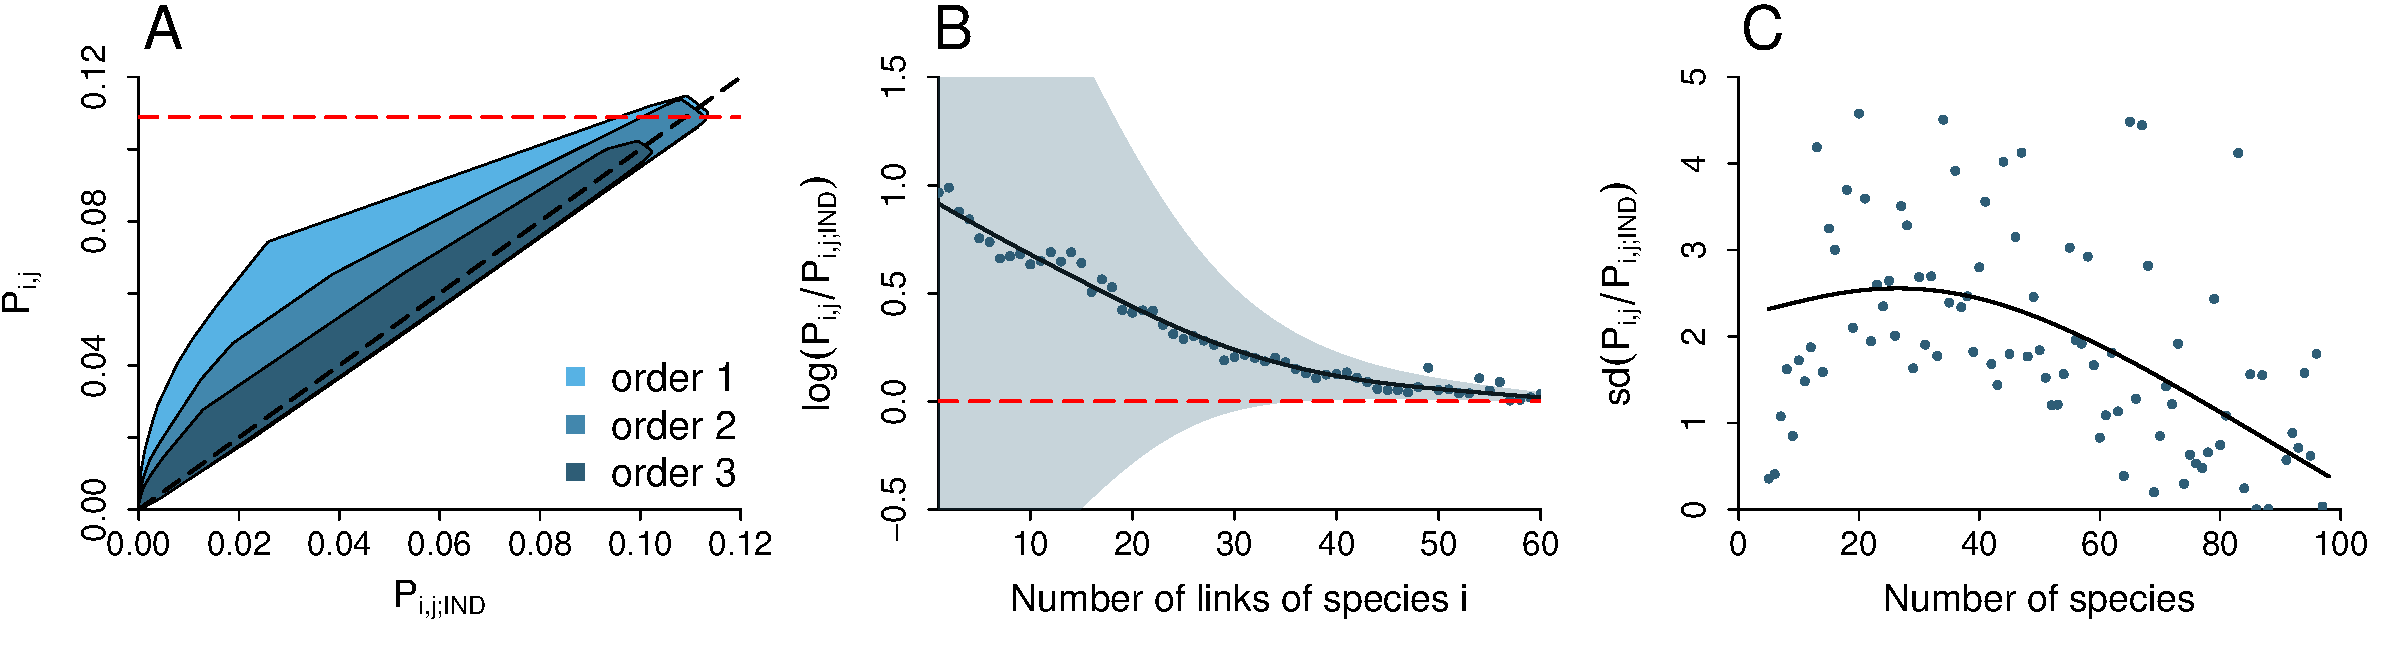
\includegraphics[width=\textwidth]{./chapitre2/fig1.eps}
\caption[Co-occurrence in multi-species networks]{Co-occurrence in multi-species networks.
(A) The disparity between observed co-occurrence ($P_{i,j}$) and independent co-occurrence ($P_{i,j;\text{IND}}$) decreases with the path length between nodes (species). The enveloppes are drawn around the 5\% and 95\% quantiles of all of the data, from 100 replicated simulations for every species richness value (5 to 100 species).
(B) The strength of co-occurrence ($log(P_{i,j}/P_{i,j;\text{IND}})$) decreases with the number of interactions of a species $i$ (\textit{i.e.} the degree of a node). Points represent the mean for a particular degree of node value (1 to 60). The solid line represents the overall trends and the grey envelopped refelcts the variance associated. At least 3000 values were used for each point.
(C) The standard deviation of the strength of association ($sd(P_{i,j}/P_{i,j;\text{IND}})$) and thus the variance decreases with species richness. Taken together, (B) and (C) imply that species distributions converge to independence with increasing species richness.}
\label{figchap2_1}
\end{figure}

\paragraph*{Distance decay of observed co-occurrence.} The distribution of
observed co-occurrence is illustrated for pairs of species separated by
different path lengths at Fig. \ref{figchap2_1} A. The observed co-occurrence is presented
as a function of the expected co-occurrence under the hypothesis of
independent distributions. The strongest associations (given by the distance
between the observed and the independent co-occurrence) are observed among
pairs of species directly interacting with each other. The variance of the
distribution reduces from direct to first order indirect interactions, and
from first-order to higher interactions. We conclude that indirect non-
independent co-occurrences are possible in complex networks, but their
magnitude decreases as the number of links between two nodes decreases. This
result is similar to the observation of a distance decay of indirect
interactions in food webs \citep{Berlow2009}.



\paragraph*{Strength of co-occurrence decreases with degree and species
richness.} We performed simulations with a gradient of species richness and
observed that the variance of observed co-occurrence also decreases with the
degree of a species, i.e. the number of direct interactions a species is experiencing
(Fig. \ref{figchap2_1} B). We illustrated the relationship between the
degree of a species and the observed co-occurrence for pairs of species with a
direct association (Fig. \ref{figchap2_1} C). This phenomenon has the consequence that the
strength of observed co-occurrence reduces with species richness. The niche
model has a constant connectance \citep{Williams2000}, which has for consequence an increase of the degree with species richness. We find that the strength of co-occurrence
decreases with the degree. This result is straightforward to interpret: the
more diverse are the interactions, the weaker the impact of each
pairwise direct interaction on the species distribution. Again, this result is
similar to the observation of a scaling relationship between pairwise
interactions and food web diversity \citep{Berlow2009}.

%---------------------------------------------
\section*{Discussion}
\label{discussion}

%
We first develop a probabilistic species distribution model constrained by
biotic interactions using conditional probabilities of co-occurrence. We then illustrate five general principles underlying the impact of ecological interactions on co-occurrence and that should be considered for the formulation of a general theory of species co-occurrence. Two of them have been widely noted before: \textbf{i)} direct interactions affect species distributions and generate deviations in co-occurrences from that expected if distributions of species were independent from each other; \textbf{ii)} the effect of direct associations is often asymmetric, as envisioned in trophic metacommunity ecology \citep{Holt2009}. We also illustrate principles that have been overlooked in most studies of co-occurrence \citep{Araujo2011}; \textbf{iii)} indirect interactions generate deviate co-occurrence from expectation under independence assumption; \textbf{iv)} the strength of indirect associations decreases with the length of the shortest path distance between species pairs in a network; while \textbf{v)} also decreasing with the number of interactions a species is experiencing. We started with the analysis of three species modules to document these principles and then showed their applicability in multi-species networks. We find that the above principles also apply in larger networks, but that the strength of pairwise associations weakens as the number of species increases.

Our results have considerable implications for interpretation of co-occurrence data. Firstly, they demonstrate the considerable variety of mechanisms causing pairwise associations. Such variety of mechanisms makes interpretation aggregated indices of co-occurrence, such as the C-score, very difficult \citep[see also][]{Araujo2014}. Previous studies already made
the argument that positive and negative interactions could balance each other
\citep{Boulangeat2012} and consequently associations should be
studied on a pairwise basis \citep{Veech2013}. At least, some
measure of the variability of the associations is required, and at best
metrics such as network analyses \citep{Araujo2011} should be used to
characterize their complex structure. But most importantly, our analyses
reveal the difficulty to infer species interactions from co-occurrence
matrices. Associations are not symmetric and, therefore, indices that are capable of dealing with them are required. Null model testing is not sufficient; significance is assessed from the difference between observed co-occurrence and co-occurrence expected under independent distributions and is, consequently, symmetric. In addition, statistically significant associations cannot be interpreted as evidence of direct interactions. Our results also show that indirect interactions, and not only second order interactions, contribute to generate apparent non-independent co-occurrence. These indirect associations could be of any kind and are impossible to detect solely based on knowledge of direct interactions.

Null models of species associations should, thus, be used only to reveal the
structure of co-occurrence data. The lack of an association between a pair of
species is no unequivocal evidence of absence of direct interactions. It must be interpreted as the absence of a net effect in the spatial co-occurrence arising from pairwise interaction alone. For instance, in the case species A is competing with species B and species C, and B with C, it is possible that A and C could be independently co-occurring if there is a strong indirect positive interaction A-C arising from the A-B and B-C direct interactions. Null model testing is consequently
subject to important type I (false interpretation of a significant
association) and type II errors (false interpretation of an absence of
association). The problem itself does not come from the statistical method per
se, the description of co-occurrence in the data will be right provided that
the technique is adequate, but from the interpretation of the null model
analysis.

Should we, therefore, abandon joint species distributions modelling (JSDM) and all of the information contained in co-distribution data? While our results might lead to such an interpretation, there is still some value in species co-occurrence data that could be used in distribution models. The appropriate use of JSDMs is to remove biases in the evaluation of species-specific relationship with the environment. Accounting for joint distribution will contribute to the evaluation of the conditional distribution of a species when all other species are absent. In other words, they should be used to improve the evaluation of the fundamental niche. The JSDMs will, however, fail to
predict the right occurrence probability of a species for communities that
have no analogue to the training dataset. JSDMs are using only the net
associations between pairs of species and are not meant to recover the direct
pairwise conditional co-occurrences. For instance, a JSDM evaluated for a plant, an herbivore and a carnivore will provide the correct description of the joint distribution of all three species, but will be of limited use to predict the distribution of the plant and the herbivore if the carnivore disappears from the system. Further developments are, consequently, required to solve the issue and account for both direct and indirect interactions. One possible solution would be to constrain JSDMs with a prior expectation of the underlying
structure of direct interactions.
%
It is also valuable to ask whether the inference of the structure of interaction
networks is feasible from the observation of co-occurrences (as they result
from many ecological processes).
There is growing interest in inferring ecological network structure from alternative sources of information \citep{Gravel2013, Morales-Castilla2015}.
This problem is challenging because of the multiple influences on co-occurrence. Our analysis of three species modules with conditional probabilities revealed it is feasible numerically, to obtain an estimate of all pairwise
conditional probabilities when accounting for higher order interactions. Known
quantities are the marginal probabilities and observed co-occurrence. The
parameters to be evaluated are all fundamental conditional probabilities,
representing the direct associations between pairs of species (the
$p_{i|j,\overline{K}}$). This is a $S \times S$ problem to solve and thus
requires a significant amount of data. It might, however, be solved with large
datasets where the number of sites $N$ is much larger than $S$. There might
also be methods to reduce the dimension of the problem because usually only a
small fraction of potential interactions are met in a network (corresponding
to the connectance $C$). While a net interaction network is likely to be fully
connected ($S\times S$ links), the direct interaction network has still only a
fraction $C$ of these links realized. Bayesian approach with latent variables
could even further help reducing the dimension of the problem \citep[\textit{e.g.}][]{Rohr2010, Ovaskainen2010}. In such methods, latent variables
are evaluated for each species to represent the underlying structure of the
ecological network. It was found that between two and four parameters per
species would be required to successfully represent more than 80\% of interactions
in a predator-prey network \citep{Rohr2010}. This approach could,
therefore, be used to represent the underlying structure of direct interactions
and to evaluate numerically the non-null conditional probabilities. Note that these pairwise direct interactions should be interpreted
specifically with reference to spatial dynamics because they would still
represent phenomenologically the consequences of interactions, not the
mechanisms of interactions.
%
The next step in the development of a theory of species co-occurrence (and of
species distribution) is the addition of environmental constraints. Our
approach assumed a homogeneous environment, mainly for tractability of
equations. We acknowledge that non-independent co-occurrence could also arise
because of  shared environmental requirements. The addition of environmental
constraints would be easy to implement in our framework by simply making the
conditional probability in absence in absence of interactions a function of
the environment. Every quantity we derive after would be conditional on the
environment. What would be more challenging but, nonetheless, feasible
numerically, would be to make the direct interaction itself a function of the
environment. There is now growing evidence that ecological interactions are
context dependent \citep{Chamberlain2014, Poisot2012}. We
view this integration as the next step to the derivation of a theory-driven
species distribution model taking into account biotic interactions \citep{Thuiller2013}.

\section{Acknowledgments}
This work was inspired by discussions with T. Poisot, D. Stouffer, A.
Cyrtwill and A. Rozenfield. Thanks to Matt Talluto and Isabelle Boulangeat for helpful comments on a previous version of the manuscript. Financial support was provided by the Canada Research Chair program
and a NSERC-Discovery grant to D. Gravel. M. Ara\'ujo acknowledges support from Imperial Colege’s Grand Challenges in Ecosystems and Environment Initiative.
